\section{Глава 1. Сбор и подготовка данных}

В данной главе будет рассмотрен способ сбора данных, краткая характеристика этих данных, а также предобработка полученных данных.

\subsection{1.1. Сбор данных}

Для сбора информации о пользователях в качестве социальной сети была выбрана социальная сеть ВКонтакте. Данная сеть является наиболее популярной в русскоязычном сегменте и ее главным преимуществом является удобный интерфейс прикладного программирования (application programming interface - API) для разработчиков. API - это интерфейс, предоставляющий набор готовых функций, процедур и классов, для удобного взаимодействия разработчиков с сервисом. 

В качестве атрибутов пользователей были выбраны следующие признаки, извлекаемые из профилей:
\begin{enumerate}
\item Пол
\item Возраст
\item Город проживания
\item Страна проживания
\item Текущая деятельность
\item Политическая принадлежность
\item Количество детей
\item Семейное положение
\item Город расположения школы
\item Год окончания школы
\item Город расположения университета
\item Год окончания университета
\item Уровень образования
\end{enumerate}

Стоит сделать замечание по поводу используемых признаков. Так, например, под городом проживания, страной проживания, городом расположения школы и университета здесь понимаются целочисленные идентификаторы. Возраст, количество детей, год окончания школы и университета принимают целочисленное значение. Все остальные атрибуты являются категориальными, а именно:
\begin{itemize}
\item Пол $\in \{\text{мужской, женский}\}$
\item Текущая деятельность $\in$ \{работа, среднее образование, высшее образование\}
\item Политические предпочтения $\in$ \{коммунистические, социалистические, умеренные, либеральные, консервативные, монархические, ультраконсервативные, индифферентные, либертарианские\}
\item Семейное положение $\in$ \{женат/замужем, не женат/не замужем, неизвестно\}
\item Уровень образования $\in$ \{среднее образование, высшее образование, неизвестно\}
\end{itemize}


Для того, чтобы загрузить информацию о профилях пользователей, а также информацию о социальном графе,  был реализован программный модуль, посредством языка python3.6, который использует API ВКонтакте \cite{API VK}. Главным ограничением API ВКонтакте является то, что он позволяет делать не более 3 запросов в секунду.

Реализованный программный модуль выполняет следующие задачи:
\begin{enumerate}
\item Случайным образом генерируются пользовательские идентификаторы 
\item Для полученного списка пользователей проверяется, указал ли он пол и возраст с помощью метода API <<users.get>>
\item Собирается информация о списке друзей, путем обращения к методу API <<friends.get>> и затем исходная выборка фильтруется на предмет того, чтобы у каждого пользователя было не менее 25 друзей
\item Для итогового списка пользователей собирается информация о профилях с помощью метода API <<users.get>>
\end{enumerate}

В итоге были получены социальные связи для 1000 пользователей и демография для 125 000.

Все данные было принято хранить в формате CSV, поскольку использование данного формата удобнее для библиотек машинного обучения и эффективнее по памяти, чем в JSON.

\subsection{1.2. Предобработка данных}

Поскольку многие методы машинного обучения, используемые в данной работе чувствительны к масштабу, а также имеется много категориальных переменных, то перед применение алгоритмов машинного обучения и нейронных сетей, исходные данные, полученные из профилей пользователей, необходимо предобработать.



\subsection*{One Hot Encoding}

One Hot Encoding -- это способ представления категориальных переменных в виде бинарных векторов. Его суть заключается в том, чтобы сопоставить каждому уникальному значению категориальной переменной двоичный столбец. 

Однако главным недостатком такого представления является то, что размер векторов растет с ростом числа уникальных значений в категориальной переменной. 

Избавиться от вышеуказанного недостатка могут помочь методы уменьшения размерности.

На Рис. \ref{fig:ohe_example} продемонстрировано использование данного метода к категориальной переменной <<Семейное положение>>.  Другие категориальные признаки обрабатывались аналогично. Обработка была выполнена с помощью метода <<get\_dummies>> библиотеки pandas \cite{pandas} 

\begin{figure}[h]
\begin{subfigure}[h]{0.4\linewidth}
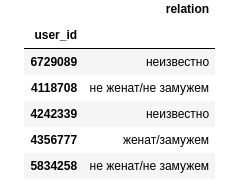
\includegraphics[width=\linewidth]{images/ohe_example1.png}
\caption{Данные до преобразования}
\end{subfigure}
\hfill
\begin{subfigure}[h]{0.6\linewidth}
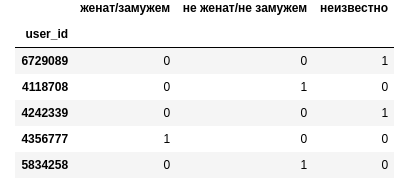
\includegraphics[width=\linewidth]{images/ohe_example2.png}
\caption{Данные после преобразования}
\end{subfigure}%
\caption{Ohe Hot Encoding}
\label{fig:ohe_example}
\end{figure}

\subsection*{Масштабирование}

Масштабирование -- это процесс изменения диапазона значений признака. Способ масштабирования, при котором каждый из признаков приводится к диапазону от 0 до 1 называется нормализацией. Другой способ масштабирования -- стандартизация. Под стандартизацией подразумевается такая предобработка данных, после которой каждый признак имеет математическое ожидание равное 0 и дисперсию равную 1.

В данной работе в качестве масштабирования был выбран процесс стандартизации, поскольку это один из самых употребляемых способов масштабирования признаков.

Стандартизация элемента выборки $x$ происходит следующим образом:
$$x' = \frac{x - \mu}{\sigma} $$
где $\mu$ - среднее значение признака, $\sigma$ - среднеквадратичное отклонение признака

\subsection{1.3. Формирование выборок}

Для решения поставленных задач были сформированы следующие выборки:
\begin{itemize}
\item Исходная -- выборка с исходными атрибутами пользователей (без преобразования)
\item Scaled -- выборка, к которой ко всем признакам была применена стандартизация
\item OHE -- выборка, к которой к категориальным признакам был использова алгоритм One Hot Encoding 
\item OHE + Scaled -- выборка, к которой сначала применили One Hot Encdoing, а затем проведена стандартизация
\end{itemize}

При этом в качестве тренировочной выборки было выбрано 80\% данных и 20\% соответственно для тестовой.   

Для методов машинного обучения с учителем, которые будут описаны в следующей главе, существует проблема переобучения. Это явление при котором построенная модель сильно подстраивается под тренировочную выборку и хорошо классифицирует примеры из этого набора, но плохо классифицирует любые другие примеры из тестовых. Это происходит вследствие того, что в процессе обучения модель выявляет закономерности в тренировочном наборе, которые отсутствуют в генеральной совокупности. 

Способы борьбы с данной проблемой зависят от выбранной модели. Однако, одним из способов, который применим ко всем методам, является кросс-валидация (перекрестная проверка). Его суть заключается в том, что имеющиеся данные разбиваются на $k$ частей. После этого на $k-1$ частях производится обучение модели, а оставшаяся часть данных используется для тестирования. Данная процедура повторяется $k$ раз, гарантирующая, что каждая из $k$ частей данных будет использоваться для тестирования.

В данной работе для предотвращения переобучения применена кросс-валидация к тренировочным данных с разбиением на 5 частей. 


\clearpage